\section{Audio Transmission Measurement}
\label{sect:Trans}
This second major category of VNA measurements consists of generating a sine wave and applying this to some form of network.
 The network must have at least two sets of connections that act as the input and output.
The transmission measurement determines the complex input and output voltages and then computes the ratio of the voltage magnitudes along with the difference in phase.
%
\subsection{Description}
\label{subsect:TDescr}
\textbf{Complex Transmission - }The concept of voltage gain  is common.
This is directly applied here when we take the ratio of the magnitude of the output voltage to that of the input voltage.
That measure does not involve the phase of the signals and is the same as applying a portable DVM to the terminals and dividing the result with a calculator.

The "complex" or "vector" part of a gain measurement results from making phase measurements in addition to magnitude measurements.
With our VNA, we determine how much phase difference there is between the input and output sine waves.
This can be important for equipment such as  filters, control systems or communications networks.
In part, it also allows a complete mathematical model of linear circuits to be constructed .  This is a valuable tool for design of circuits.

It is worth noting that some of the common Radio Frequency concepts such as scattering parameters and reflection coefficients are also applicable at low frequencies.  Complex transmission (and impedance) measurements support these descriptors.  We won't attempt to cover all the possibilities here, but it would be an interesting topic for someone to explore.

\subsection{Instructions}
\label{subsect:TInstr}
\textbf{Single Frequency Measurements - }This procedure parallels the impedance measurements of the previous section.
We will cover the essence of a transmission measurement using the touch screen.
Everything covered here, and more, can be done via the USB-Serial link, as is described in the "AVNA Serial Control" section.

When the AVNA is powered up, as shown in  Figure \ref{AVNA_000-label},  you have a choice of four Audio Test Instruments along with Service and Calibration functions.  As was the case for impedance measurements, we again select "AVNA" as our instrument.  The next screen, Figure  \ref{AVNA_001-label}, applies to both impedance and transmission measurements and allow us to select single or swept frequency measurements as well as to change the source resistance between 50 and 5000 Ohms.  First, check if the reference resistance is set to 50 Ohms and that the input resistance switch has the 50-Ohm termination resistor on.  This sets us up for a common 50-Ohm in and out transmission measurement.

To continue with the sample transmission measurement, we will select "Single Freq."  At this point we select the frequency of measurement using the "Freq Down" and "Freq Up"  buttons.  We will suppose our frequency of interest is 5000 Hz and we will use the buttons to set that.  Now, tap on "Meas T' to be ready for transmission measurements.   At this point, the AVNA will warn us that a Cal is needed as seen on the next screen, Figure  \ref{AVNA_043-label}.
\begin{figure}[H]
\begin{center}
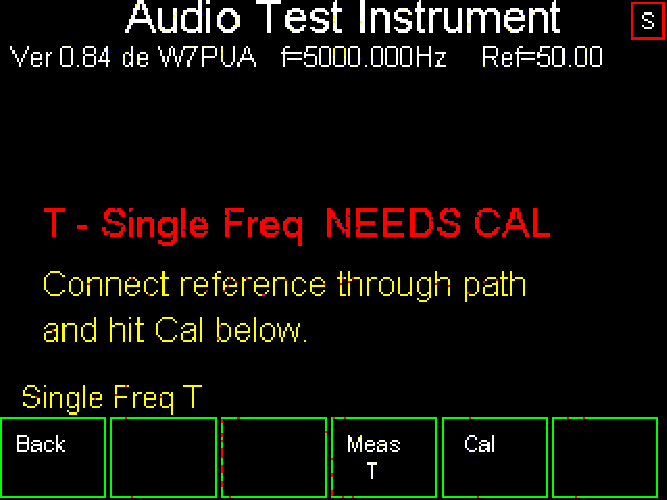
\includegraphics[scale=0.75]{./images/AVNA_043.pdf}
\caption{AVNA Transmission showing need for calibration.}
\label{AVNA_043-label}
\end{center}
\end{figure}
%
 We will proceed to Cal by placing a wire between the hot Z and T terminals and tapping "Cal" at the bottom.   There is a brief delay, a brief message and then the almost blank screen seen here.
\begin{figure}[H]
\begin{center}
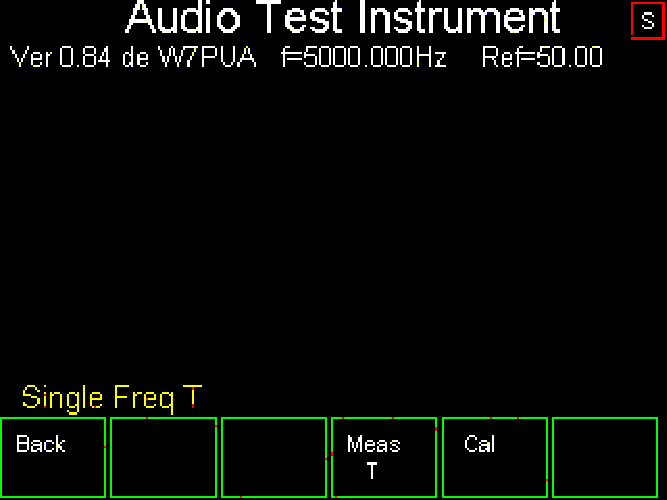
\includegraphics[scale=0.75]{./images/AVNA_044.pdf}
\caption{Transmission measurement after calibration.}
\label{AVNA_044-label}
\end{center}
\end{figure}
%
This means the transmission path is calibrated at this one frequency and ready to use.  Before removing the calibration wire, tap on the "Meas T" button to confirm that the Gain is 0.0 dB and the phase is 0.0 degrees for the direct connection.  The screen should look very much like the following, Figure \ref{AVNA_033-label} or the problem should be tracked down.  We can redo the "Cal" if needed.  Otherwise, it is time to connect up a circuit and measure it.
\begin{figure}[H]
\begin{center}
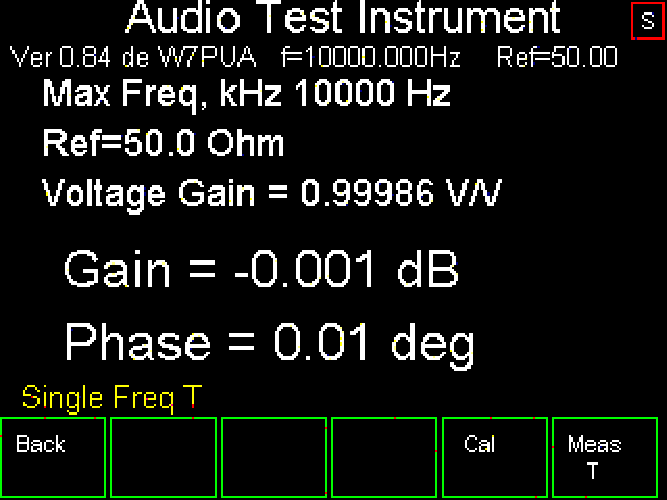
\includegraphics[scale=0.75]{./images/AVNA_033.pdf}
\caption{Single frequency Transmission measurement with the calibration jumper still in place.}
\label{AVNA_033-label}
\end{center}
\end{figure}
%
When measuring impedances, I used a series combination of a 10 Ohm resistor and a 0.22 $\mu$F capacitor.  This time, for a transmission measurement, the two parts will be connected between the hot Z and T terminals. This replaces the wire used for calibration.  This is not a particularly interesting circuit to test, but it illustrates the measurement.  For single frequency measurements, the screen will update about once a second.  This is useful for testing multiple components, or when making adjustments.  Here is the result of my measurement for this RC network.
\begin{figure}[H]
\begin{center}
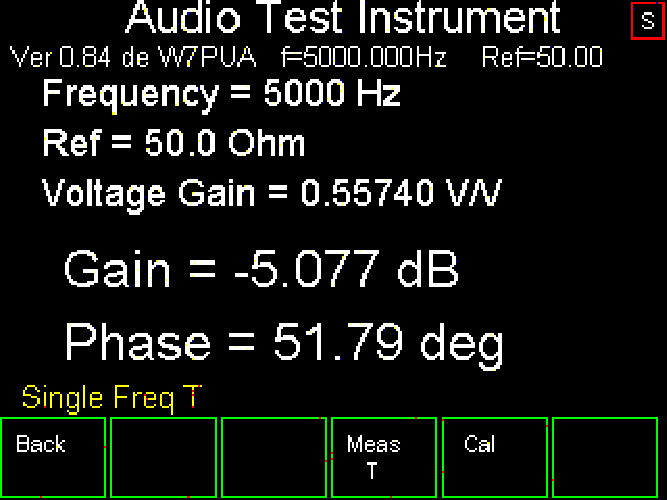
\includegraphics[scale=0.75]{./images/AVNA_047.pdf}
\caption{AVNA Transmission measurement for a single frequency.}
\label{AVNA_047-label}
\end{center}
\end{figure}
%
For the measurements  just made, the source and termination impedances were both 50-Ohms.  This is the way we often measure components at frequencies above the range of our AVNA.  But, we have several other impedance options available that can be useful.  If we use the BNC connector instead of the terminals, the source impedance will be much lower, typically less than an Ohm  Also if we move the switch to not use the 50-Ohm input termination, the measuring input impedance will be 1.0 megohm in parallel with about 25 pF.  This is a common setup for low frequency testing,  It is also compatible with many oscilloscope probes.  Remember that if we change any of the source or termination impedances we need to do a new calibration.  Also, changing either of these two impedances will change the transmission measurement values, sometimes by a large amount.

\textbf{Swept Frequency Measurements - } Just a we did for impedance measurements we can utilize a built-in set of frequencies to measure transmission amplitude and phase.  The same 13 frequencies are available covering 10 to 40,000 Hz.  Under Serial Control, this same measurement can be made at an arbitrary set of frequencies (see AVNA Serial below).

The procedure parallels that of Single Frequency measurements, and so we won't repeat every detail.  Please look back to the previous section of Single Frequency Measurements  for additional information.  We start from the main AVNA screen, Figure \ref{AVNA_001-label} where we can again select the source resistance and then select "Sweep."  At his point we can choose "Meas T" from the bottom menus.  Again, we will have a bold message reminding us to do a "Cal."  You connect a wire or short test clip between the top terminals and tap on "Cal."  After  about 10-seconds the middle of the screen is  blank and the circuit to be measured  should be connected in place of the calibration wire.  Tapping on "Single T Sweep" and waiting about 8-seconds should produce a similar screen to Figure  \ref{AVNA_032-label}, seen here.
\begin{figure}[H]
\begin{center}
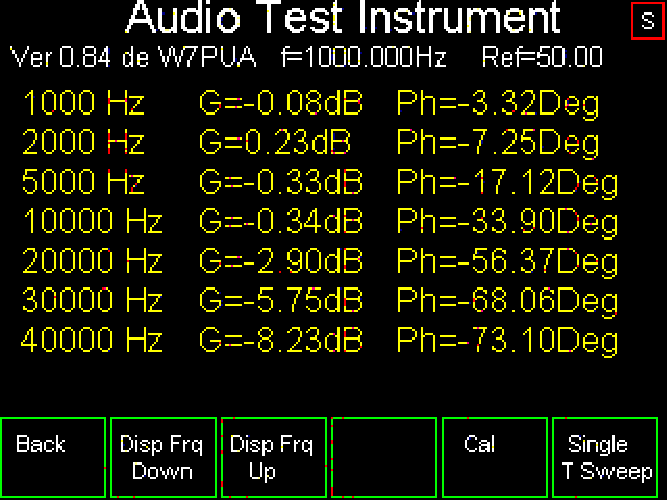
\includegraphics[scale=0.75]{./images/AVNA_032.pdf}
\caption{AVNA Swept frequency Transmission measurement screen.}
\label{AVNA_032-label}
\end{center}
\end{figure}
%
All 13 measurements have been made, but only 7 are displayed on the screen.  Use the bottom buttons, "Disp Frq Up" and "Disp Frq Down" to display the, the range of interest.  When you change the circuit and want to re sweep, again tap "Single T Sweep" and wait a few seconds for the new results.  You can also go back to recalibrate at any time by connecting a through jumper wire and tapping "Cal."

%
\subsection{Discussion}
\label{subsect:TDiscus}
The calibration measures the voltage magnitude and phase with the signal source connected to the voltmeter.  This is saved and used for following circuit transmission measurements.  For that, the ratio of the new voltage magnitude to the calibrate magnitude is used to find the relative transmission magnitude.  Similarly, the calibrate phase is subtracted from the new measurement phase.  If the calibrate jumper wire is still in place, this gives a relative  transmission magnitude of 1.000 and a measurement phase of 0.000 degrees.

Averaging is built into these measurements to decrease the noise observed.  This increases the accuracy at higher amounts of attenuation.  It is inherent that lower frequencies take longer amounts of time.  For our lowest frequency of 10 Hz, each cycle requires 0.1 seconds.  The averaging algorithm used requires integral numbers of cycles, and the time adds up.
